%% ****** Start of file apstemplate.tex ****** %
%%
%%
%%   This file is part of the APS files in the REVTeX 4.2 distribution.
%%   Version 4.2a of REVTeX, January, 2015
%%
%%
%%   Copyright (c) 2015 The American Physical Society.
%%
%%   See the REVTeX 4 README file for restrictions and more information.
%%
%
% This is a template for producing manuscripts for use with REVTEX 4.2
% Copy this file to another name and then work on that file.
% That way, you always have this original template file to use.
%
% Group addresses by affiliation; use superscriptaddress for long
% author lists, or if there are many overlapping affiliations.
% For Phys. Rev. appearance, change preprint to twocolumn.
% Choose pra, prb, prc, prd, pre, prl, prstab, prstper, or rmp for journal
%  Add 'draft' option to mark overfull boxes with black boxes
%  Add 'showkeys' option to make keywords appear
%\documentclass[twocolumn]{article}
%\documentclass[aps,prl,preprint,groupedaddress]{revtex4-2}
%\documentclass[aps,prl,preprint,superscriptaddress]{revtex4-2}
\documentclass[aps,prl,reprint,superscriptaddress, onecolumn, 11pt]{revtex4-2}

% \usepackage[margin=1in]{geometry}

\usepackage[T1]{fontenc}
% Mathbb digits
\usepackage{bbm}

\usepackage{tikz}
\usetikzlibrary[graphs]

% You should use BibTeX and apsrev.bst for references
% Choosing a journal automatically selects the correct APS
% BibTeX style file (bst file), so only uncomment the line
% below if necessary.
\bibliographystyle{apsrev4-1}

% Modify section headers
\usepackage{titlesec}
% Restore original section header (approximately)
\titleformat{\section}[block]{\bfseries}{\thesection}{5pt}{\filcenter\MakeUppercase}{}
\titlespacing*{\section}{0pt}{*4}{*2}
% Make subsection headers bold, smallcaps, and inline
\titleformat{\subsection}[runin]{\bfseries}{\thesubsection}{5pt}{\scshape}{}
\titlespacing*{\subsection}{0pt}{*1}{*2}

%\usepackage[toc,title,page]{appendix}

\usepackage{graphicx}
\graphicspath{{img/}}

\usepackage{amssymb,amsmath,amsthm}

% Ani macros
\newcommand{\paren}[1]{\left(#1\right)}
\newcommand{\brac}[1]{\left[#1\right]}
\newcommand{\curly}[1]{\left\{#1\right\}}
\newcommand{\mc}[1]{\mathcal{#1}}
\newcommand{\braket}[2]{\langle #1|#2 \rangle}
\newcommand{\cbra}[1]{(#1|}
\newcommand{\cket}[1]{|#1)}
\newcommand{\bracket}[2]{(#1|#2)}
\newcommand{\suml}[3]{\sum_{#1}^{#2}#3}
\newcommand{\prodl}[3]{\prod_{#1}^{#2}#3}
\newcommand{\intl}[3]{\int_{#1}^{#2}#3}
\newcommand{\pr}[0]{^\prime}
\newcommand{\mb}[1]{\mathbf{#1}}
\newcommand{\dg}[0]{^\dagger}
\newcommand{\dd}[0]{\text{d}}
\newcommand{\dv}[2][]{\frac{\text{d}#1}{\text{d}#2}}
\newcommand{\pdv}[2][]{\frac{\partial#1}{\partial#2}}
\newcommand{\mbb}[1]{\mathbbm{#1}}
\newcommand{\str}[1]{\boldsymbol{\mathbf{#1}}}
\newcommand{\prob}[0]{\text{Pr}}
\newcommand{\wtil}[1]{\widetilde{#1}}
\newcommand{\vac}[0]{\ket{\mathrm{vac}}}
\newcommand{\swap}[0]{{\textsc{swap}}}
\newcommand{\px}[1]{\sigma^{x}_{#1}}
\newcommand{\py}[1]{\sigma^{y}_{#1}}
\newcommand{\pz}[1]{\sigma^{z}_{#1}}
\newcommand{\pplus}[1]{\sigma^{+}_{#1}}
\newcommand{\pminus}[1]{\sigma^{-}_{#1}}
\newcommand{\ha}[0]{\ensuremath{H}}
\newcommand{\hj}[0]{\ensuremath{H_{J}}}
\newcommand{\hh}[0]{\ensuremath{H_{h}}}
\newcommand{\uti}[0]{\ensuremath{U}}
\newcommand{\utd}[0]{\ensuremath{V}}
\newcommand*{\tran}{^{\mkern-1.5mu\mathsf{T}}} % transpose
\newcommand*{\idm}{\ensuremath{\mathbbm{1}}}
\renewcommand{\vec}[1]{\ensuremath{\boldsymbol{#1}}}
\newcommand{\cis}[0]{\ensuremath{\Pi}}

\newcommand{\iten}[0]{\texttt{itensor}}

% Math commands
\usepackage{mathtools}
\mathtoolsset{centercolon}
\DeclareMathOperator{\poly}{poly}
\DeclareMathOperator{\degree}{deg}
\DeclareMathOperator{\dom}{dom}
\DeclareMathOperator{\image}{image}
\DeclareMathOperator{\id}{id}
\DeclareMathOperator{\Sym}{Sym}
\DeclareMathOperator{\diag}{diag}
\DeclareMathOperator{\hammingweight}{ham}
\DeclareMathOperator{\rt}{rt}
\DeclareMathOperator{\qrt}{qrt}
\DeclareMathOperator{\urt}{urt}
\DeclareMathOperator{\hqrt}{hqrt}
\DeclareMathOperator{\rs}{rs}
\DeclareMathOperator{\qrs}{qrs}
\DeclareMathOperator{\twoqubitgate}{tg}
\DeclareMathOperator{\diam}{diam}
\DeclareMathOperator{\depth}{depth}
\DeclareMathOperator{\vol}{vol}
\DeclareMathOperator{\Ex}{\symbf{E}}
\DeclareMathOperator{\Prob}{P}
\DeclareMathOperator{\tr}{Tr}
\DeclareMathOperator{\revfull}{R}
\DeclareMathOperator{\entanglementOp}{E}
\DeclareMathOperator*{\argmax}{arg\,max}
\DeclareMathOperator*{\argmin}{arg\,min}
% \DeclareMathOperator{\idm}{\symbf{1}}
\DeclarePairedDelimiter\ceil{\lceil}{\rceil}
\DeclarePairedDelimiter\floor{\lfloor}{\rfloor}
\DeclarePairedDelimiter\bra{\langle}{\vert}
\DeclarePairedDelimiter\ket{\vert}{\rangle}
\DeclarePairedDelimiter\set{\{}{\}}
\DeclarePairedDelimiter\abs{\lvert}{\rvert}
\DeclarePairedDelimiter{\norm}{\lVert}{\rVert}
\DeclarePairedDelimiterXPP\tg[1]{\twoqubitgate}{(}{)}{}{#1}
\DeclarePairedDelimiterXPP\bigo[1]{O}{(}{)}{}{#1}
\DeclarePairedDelimiterXPP\bigomega[1]{\Omega}{(}{)}{}{#1}
\DeclarePairedDelimiterXPP\diagonal[1]{\diag}{(}{)}{}{#1}
\DeclarePairedDelimiterXPP\hamming[1]{\hammingweight}{(}{)}{}{#1}
\DeclarePairedDelimiterXPP\rnumber[1]{\rt}{(}{)}{}{#1}
\DeclarePairedDelimiterXPP\qrnumber[1]{\qrt}{(}{)}{}{#1}
\DeclarePairedDelimiterXPP\hrnumber[1]{\hqrt}{(}{)}{}{#1}
\DeclarePairedDelimiterXPP\rsize[1]{\rs}{(}{)}{}{#1}
\DeclarePairedDelimiterXPP\qrsize[1]{\qrs}{(}{)}{}{#1}
\DeclarePairedDelimiterXPP\hierprod[2]{Π_{#1}}{(}{)}{}{#2}
\DeclarePairedDelimiterXPP\modular[1]{M_G}{(}{)}{}{#1}
\DeclarePairedDelimiterXPP\probability[1]{\Prob}{[}{]}{}{#1}
\DeclarePairedDelimiterXPP\expectation[1]{\Ex}{[}{]}{}{#1}
\DeclarePairedDelimiterXPP\entanglement[1]{\entanglementOp}{(}{)}{}{#1}
\DeclarePairedDelimiterXPP\rev[1]{R}{[}{]}{}{#1}
%\DeclarePairedDelimiterXPP\parstring[1]{Z}{[}{]}{}{#1}

% Better tables
\usepackage{booktabs}

\usepackage[colorinlistoftodos]{todonotes}
\newcommand{\todoi}[2][]{\todo[inline,#1]{#2}} %Macro for todo inline

%Link colors
\usepackage{color}
\usepackage{xcolor}
\definecolor{dark-red}{rgb}{0.4,0.15,0.15}
\definecolor{dark-blue}{rgb}{0.15,0.15,0.4}
\definecolor{medium-blue}{rgb}{0,0,0.5}

\definecolor{mycomment}{rgb}{0.3,0.7,0.8}
\definecolor{mygray}{rgb}{0.5,0.5,0.5}
\definecolor{lightgray}{rgb}{0.95,0.95,0.95}
\definecolor{mymauve}{rgb}{0.58,0,0.82}

\usepackage{hyperref}
\hypersetup{%
	breaklinks=true,
	% bookmarks=true,
	colorlinks,
	linkcolor={dark-blue},
	citecolor={dark-blue},
	urlcolor={medium-blue},
	pdfauthor = {Aniruddha Bapat},
	pdftitle ={Simulating the Schwinger model via matrix product states},
	pdfpagemode=UseOutlines,
	pdfborder={0 0 0}
}

% References, load last.
\usepackage[nameinlink,capitalise]{cleveref}
\crefname{figure}{Figure}{Figures}
\crefname{equation}{}{} % Do not print "Eq."
\Crefname{equation}{Equation}{Equations}

% Theorems, load after cleveref.
\newtheorem{theorem}{Theorem}
\newtheorem{lemma}[theorem]{Lemma}
\newtheorem{corollary}[theorem]{Corollary}
\theoremstyle{definition}
\newtheorem{definition}[theorem]{Definition}
\theoremstyle{definition}
\newtheorem{protocol}[theorem]{Protocol}
\crefname{protocol}{Protocol}{Protocols}



% User comments coded by color
\newcommand{\ani}[2]{\textcolor{cyan}{\emph{#1}[Ani: #2]}}

\begin{document}

% Use the \preprint command to place your local institutional report
% number in the upper righthand corner of the title page in preprint mode.
% Multiple \preprint commands are allowed.
% Use the 'preprintnumbers' class option to override journal defaults
% to display numbers if necessary
%\preprint{}

%Title of paper
\title{Simulating the Schwinger model via matrix product states}

% repeat the \author .. \affiliation  etc. as needed
% \email, \thanks, \homepage, \altaffiliation all apply to the current
% author. Explanatory text should go in the []'s, actual e-mail
% address or url should go in the {}'s for \email and \homepage.
% Please use the appropriate macro foreach each type of information

% \affiliation command applies to all authors since the last
% \affiliation command. The \affiliation command should follow the
% other information
% \affiliation can be followed by \email, \homepage, \thanks as well.
\author{Aniruddha Bapat}
\email{ani@umd.edu}
\affiliation{Joint Center for Quantum Information and Computer Science, NIST/University of Maryland, College Park, Maryland 20742, USA}
\affiliation{Joint Quantum Institute, NIST/University of Maryland, College Park, Maryland 20742, USA}
%\homepage[]{Your web page}
%\thanks{}

%Collaboration name if desired (requires use of superscriptaddress
%option in \documentclass). \noaffiliation is required (may also be
%used with the \author command).
%\collaboration can be followed by \email, \homepage, \thanks as well.
%\collaboration{}
%\noaffiliation

\date{\today}

\begin{abstract}
\end{abstract}

\maketitle
The massive Schwinger model describes 1+1D QED with one flavor of fermionic particles of mass $m$. The theory interacts via a $U(1)$ gauge field with coupling $g$. In the Kogut-Susskind formulation (and in axial gauge $A_0=0$), the model is discretized into a lattice with spacing $a$ consisting of alternating odd and even sites that each hold one component of the fermion field (electron and positron, respectively). We will adopt a serial numbering of sites and links, so that sites get odd numbers while links get even numbers (see~\cref{fig:lattice}).

\begin{figure}[h]
  \centering
  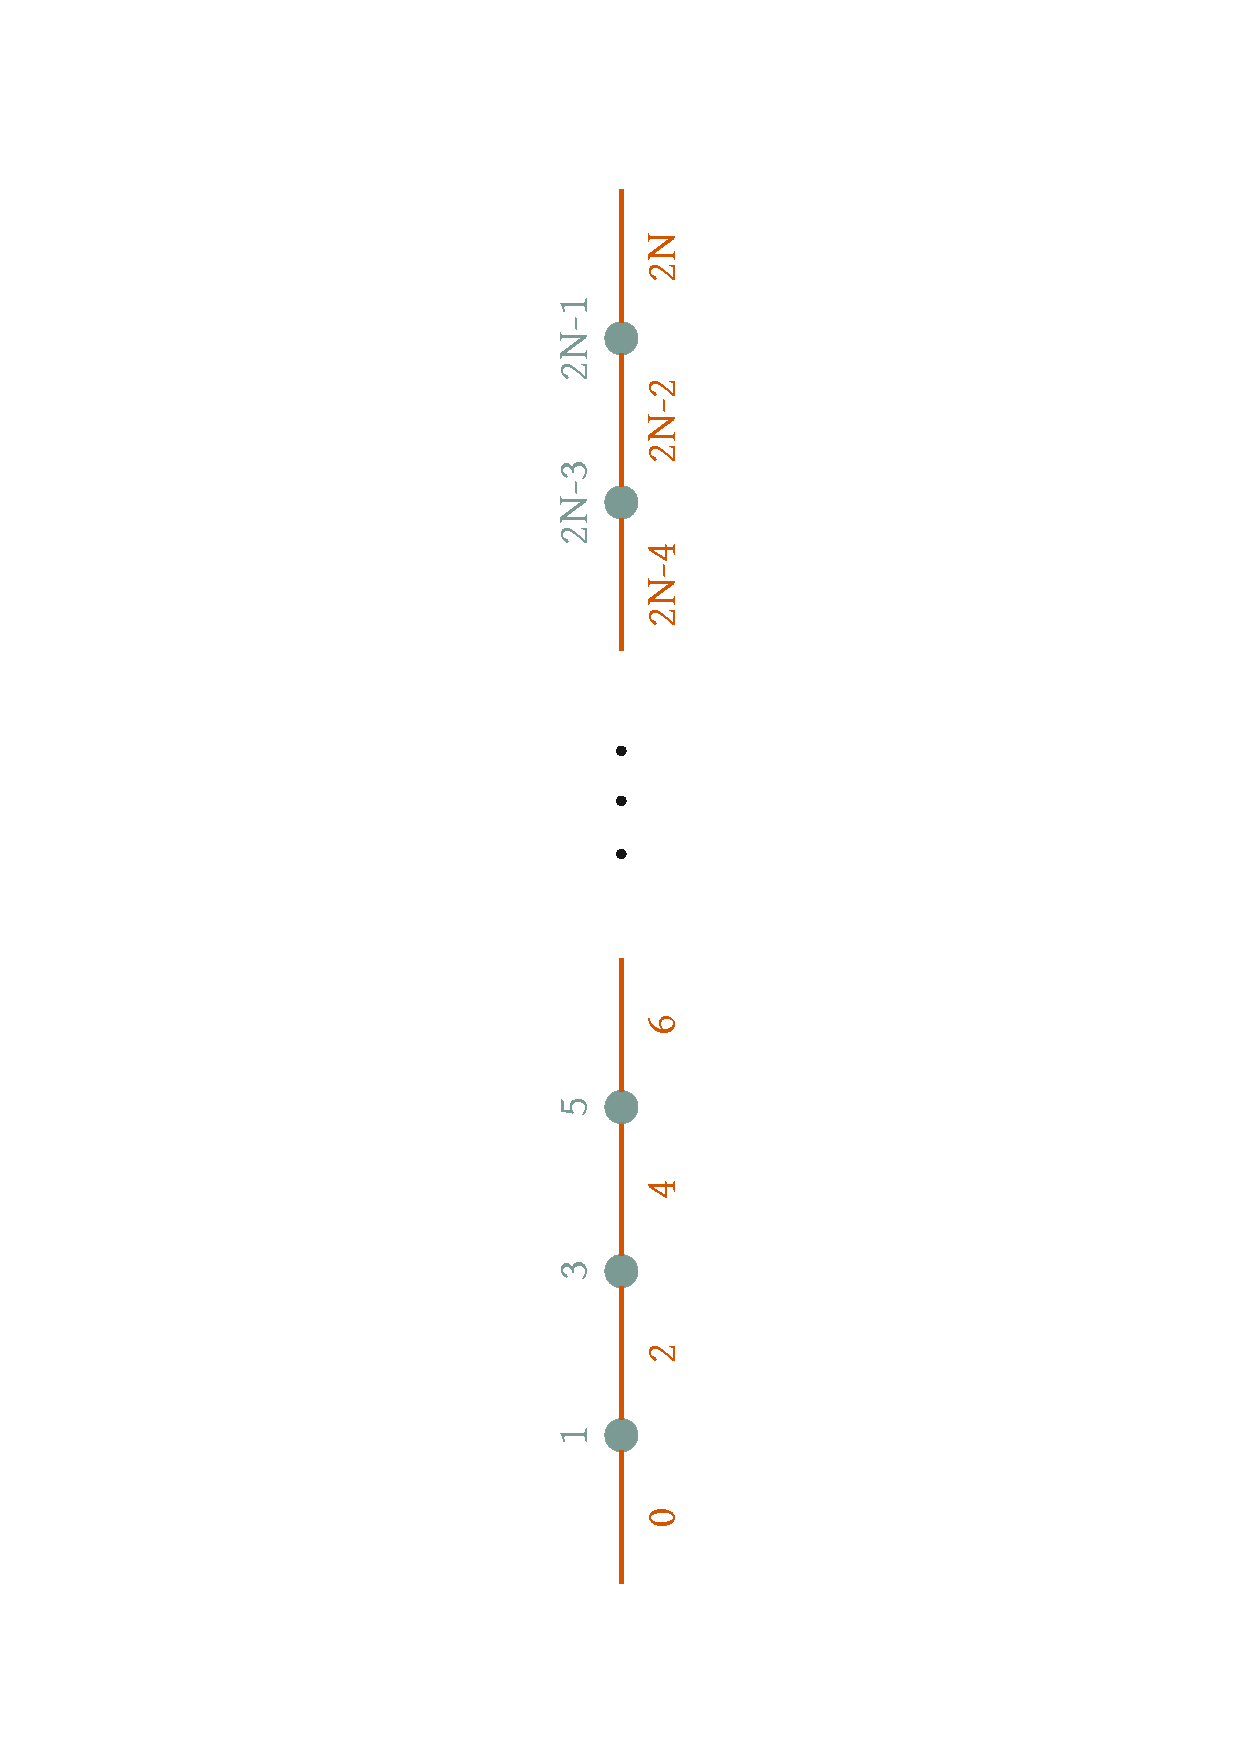
\includegraphics[angle=-90, clip=true, trim=200 0 200 0,  width=\linewidth]{lattice.pdf}
  \caption{The lattice}
  \label{fig:lattice}
\end{figure}
Under a Jordan-Wigner transformation, the Hamiltonian on $N$ matter sites (with open boundary conditions) takes on the form
\begin{equation}
  \label{eq:schwingerH}
  H = \frac{g}{2\sqrt{x}}\paren{\suml{i=1}{N}{E_{2i}^2} + \frac{\mu}{2}\suml{i=1}{N}{\frac{1 + (-1)^i\pz{2i-1}}{2}} + x\suml{i=1}{N-1}{\paren{\pplus{2i-1} U_{2i} \pminus{2i+1} +\mathrm{ h.c.}}}}\, ,
\end{equation}
where we introduced dimensionless quantities $x \coloneqq \frac{1}{g^2a^2}$ and $\mu\coloneqq \frac{2m}{g^2a}$ (in units of  $\hbar = c = 1$). In the above equation, $E_{2i}$ is the electric field at link $2i$, and $U_{2i}$ is the canonically conjugate unitary to $E_{2i}$ that satisfies $[U_{2i}, E_{2i}] = U_{2i}$. To simplify notation, we define the number operator for each matter site as $n_{2i-1}\coloneqq \frac{1 + (-1)^i\pz{2i-1}}{2}$. Extrapolating the theory to continuum is carried out in two steps. The bulk limit involves sending number of sites $N\rightarrow\infty$. Next, the continuum limit corresponds to a vanishing lattice spacing, or $x\rightarrow \infty$. In order to avoid a singularity, the limits must be carried out in the order prescribed, first $N$ and then $x$~\cite{byrnes2003, hamer1982}. 

Due to the lack of the temporal gauge term, the physical Hilbert space is specified by imposing an additional local gauge symmetry, namely, Gauss' law:
\begin{equation}
  \label{eq:gaussLaw}
  G_i \coloneqq E_{2i+2} - E_{2i} - (-1)^in_i\, .
\end{equation}
In the electric field basis $\curly{\ket{\epsilon}, \epsilon\in\mathbb{Z}}$, the gauge operator $U$ can be represented as a ``clock'' unitary $U = \suml{\epsilon\in\mathbb{Z}}{}{\ket{\epsilon}\bra{\epsilon+1}}$. It can be checked that
\begin{equation}
  \label{eq:commutationcheck}
  UE - EU = \suml{}{}{(\epsilon+1-\epsilon)\ket{\epsilon}\bra{\epsilon+1}} = U.
\end{equation}
We will use the \iten{} package~\cite{itensor} to simulate the ground state of the Schwinger model using matrix product states (MPS).

\section{Setup}
\label{sec:setup}
In \iten{}, a local Hilbert space and some in-built operators can be specified by a \emph{site set}. For example, for a lattice of spin-half particles, a site set known as ``SpinHalf'' creates a two-dimensional local Hilbert space and comes with spin operators tagged as ``Sx'', ``S+'', etc. Custom site sets can be created using the given templates.

For the Schwinger model, the matter sites can be modeled as a spin-half site, while the gauge link is modeled as a truncated bosonic site. We call such a site a ``ladder'', and truncate symmetrically to field eigenvalues $|\epsilon|\le \epsilon_{max}$. The truncated operator $U$ is then
\begin{equation}
  \label{eq:truncatedU}
  \bar{U} \coloneqq \suml{\epsilon=-\epsilon_{max}}{\epsilon_{max}-1}{\ket{\epsilon}\bra{\epsilon+1}}.
\end{equation}

We impose the global $U(1)$ symmetry $n \coloneqq \suml{i=0}{N-1}{n_{2i+1}}$ on the MPS. It is currently unknown to us whether gauge symmetries can also be used to constrain the block structure in \iten{}. In order to ensure that the final ground state ansatz lies in the physical space (i.e. satisfies Gauss law) we pick an initial state that satisfies Gauss law.

The MPS simulation now has several tunable parameters, which we summarize below:
\begin{enumerate}
\item Electric field cutoff $\epsilon_{max}$. This determines the number of dimensions in the link Hilbert space ($2\epsilon_{max}+1$) and introduces an error in the ansatz.
\item Number of matter sites $N$.
\item Lattice spacing parameter $x$.
\item Mass parameter $\mu$.
\item Maximum bond dimension $D$.
\end{enumerate}

\section{Electric field truncation}
\label{sec:Etruncation}

We study the effect of electric field truncation on the ground state energy.

\begin{acknowledgments}
Calculations were performed using the ITensor Library~\cite{itensor}.
\end{acknowledgments}

\bibliography{bibliography}
\end{document}